\documentclass{article}
\usepackage{polski}
\usepackage[utf8]{inputenc}
\usepackage{graphicx}
\usepackage{tabto}
\usepackage{hyperref}
%s\usepackage[margin=2.5cm]{geomtry}

\usepackage{graphicx}    % Pakiet pozwalający ,,wklejać'' grafikę...
\usepackage{subcaption}
\usepackage{amsmath,amssymb,amsfonts,amsthm,mathtools}
                               % Dołączamy zestaw różnych przydatnych znaczków ...
\DeclareMathOperator{\arccosh}{arccosh}
% dane autora
\author{Wiktor Pilarczyk}
\title{Warsztaty - L3 - SK\\\large{Prowadzący: Tomasz Wierzbicki}}
\date{\today}
% początek dokumentu
\begin{document}
\maketitle
\section{Wstępna konfiguracja sieci}
\subsection{Ustawienia virtualbox'a}
W VirtualBox'ie stworzyłem 4 maszyn wirtualnych z ustawieniami sieci:\\
\tabto{0.4cm}Virbian1:\\
\tabto{0.8cm}    Adapter 1 - Internal Network - local0
\tabto{0.4cm}Virbian2:\\
\tabto{0.8cm}    Adapter 1 - Internal Network - local0
\tabto{0.4cm}Virbian3:\\
\tabto{0.8cm}    Adapter 1 - Internal Network - local0
\tabto{0.8cm}    Adapter 2 - Internal Network - local1
\tabto{0.4cm}Virbian4:\\
\tabto{0.8cm}    Adapter 1 - Internal Network - local1
\newpage
\subsection{Ustawienia sieci}
Komendy użyte do konfiguracji sieci dla poszczególnej maszyny wirtualnej (po wcześniejszym sprawdzeniu adresów MAC w ustawieniach i interfejsów za pomocą 'ip link'):
\tabto{0.4cm}Virbian1:
\tabto{0.8cm}    sudo ip link set enp0s3 name enp0
\tabto{0.8cm}    sudo ip link set up dev enp0
\tabto{0.8cm}    sudo ip addr add dev enp0 192.168.1.1/24
\tabto{0.4cm}Virbian2:
\tabto{0.8cm}    sudo ip link set enp0s3 name enp0
\tabto{0.8cm}    sudo ip link set up dev enp0
\tabto{0.8cm}    sudo ip addr add dev enp0 192.168.1.2/24
\tabto{0.4cm}Virbian3:
\tabto{0.8cm}    sudo ip link set enp0s3 name enp0
\tabto{0.8cm}    sudo ip link set enp0s8 name enp1
\tabto{0.8cm}    sudo ip link set up dev enp0
\tabto{0.8cm}    sudo ip link set up dev enp1
\tabto{0.8cm}    sudo ip addr add dev enp0 192.168.1.3/24
\tabto{0.8cm}    sudo ip addr add dev enp1 192.168.2.1/24
\tabto{0.4cm}Virbian4:
\tabto{0.8cm}    sudo ip link set enp0s3 name enp-out
\tabto{0.8cm}    sudo ip link set up dev enp-out
\tabto{0.8cm}    sudo ip addr add dev enp-out 192.168.2.2/24
\\
Po wszystkich instrukcjach warto sprawdzić czy się nie popełniono błedu komendą 'ip addr'.
\\
Komputery z tej samej sieci są osiągalne za pomocą komendy 'ping'.
\subsection{Ustawianie domyślnej trasy}
Komendy użyte do ustawienia domyślnej trasy dla:
\tabto{0.4cm}Virbian1 przebiegająca przez Virbian2:
\tabto{0.8cm}    sudo ip route add default via 192.168.1.2
\tabto{0.4cm}Virbian2 przebiegająca przez Virbian3:
\tabto{0.8cm}    sudo ip route add default via 192.168.1.3
\tabto{0.4cm}Virbian4 przebiegająca przez Virbian3:
\tabto{0.8cm}    sudo ip route add default via 192.168.2.1
\\
Po wszystkich instrukcjach warto sprawdzić czysię nie popełniono błędu komendą 'ip route'.

\section{Odpowiedzi}

\begin{figure}[!htb]
\centering
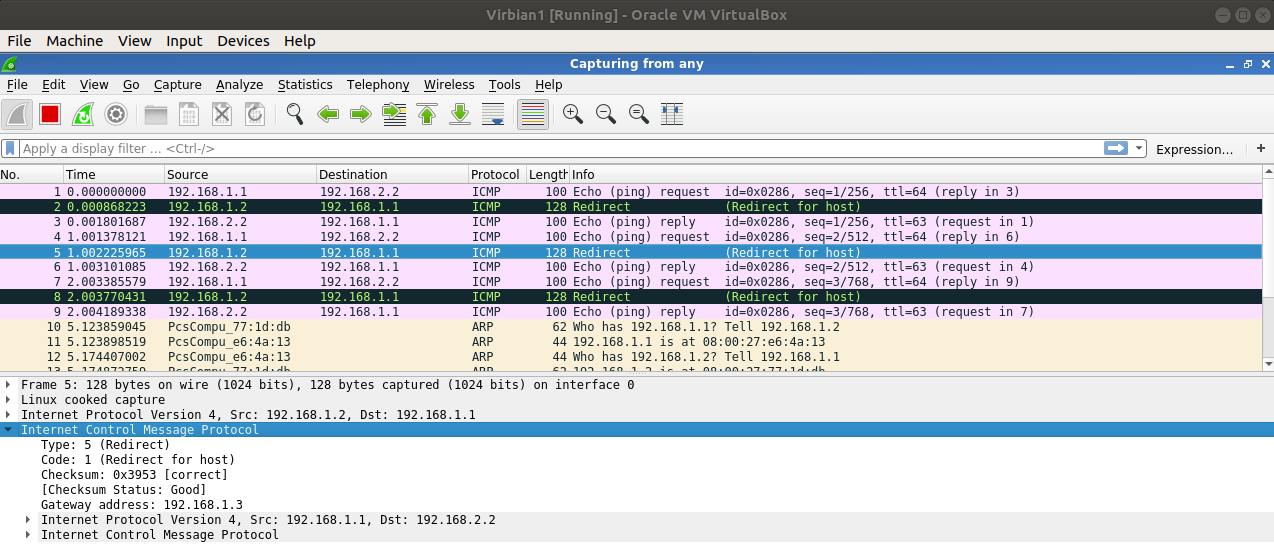
\includegraphics[width=11cm,height=5cm]{v1.png}
\caption{Wireshark dla Virbian1}
\end{figure}

\begin{figure}[!htb]
\centering
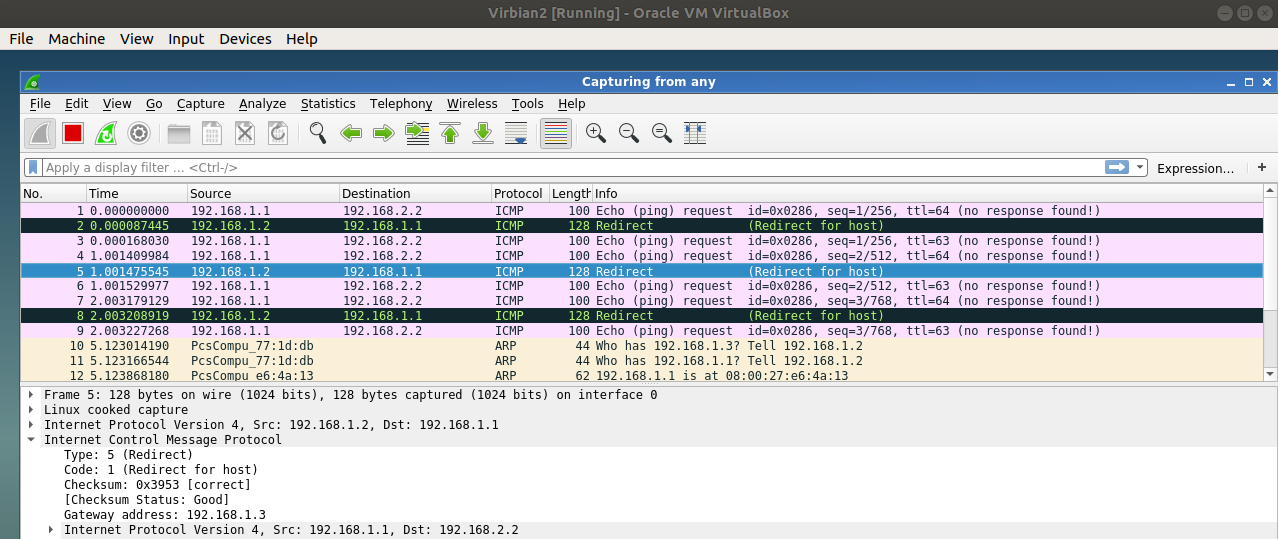
\includegraphics[width=11cm,height=5cm]{v2.png}
\caption{Wireshark dla Virbian2}
\end{figure}
\subsection{Jaka jest sugerowana przez maszynę Virbian2 modyfikacja tablicy routingu na maszynie Virbian1?}
Aby wysyłając z 192.168.1.1 do 192.168.2.2 wysyłać bezpośrednio przez 192.168.1.3 [Gateway address: 192.168.1.3] zamiast przez Virbian2 - 192.168.1.2.
\subsection{Dlaczego taka zmiana ma sens?}
Ponieważ 192.168.1.3 i 192.168.1.2 znajdują się w tej samej sieci, więc 192.168.1.1 może też wysłać wiadomość przez 192.168.1.3, przez co wiadomość dotrze szybciej i efektywniej nie korzystając z dodatkowego łącza.
\subsection{W jaki sposób maszyna Virbian2 mogła wykryć powyższy problem?}
Z faktu, że z nagłówka mogła odczytać skąd przyszedł pakiet i dokąd został przekierowany, a późniejszym sprawdzeniu czy należą do tej samej siec.

``If G2`` [u nas V3 to G2] ``and the host identified by the internet source address of the datagram are on the same network, a redirect message is sent to the host.`` \href{https://www.cisco.com/c/en/us/support/docs/ios-nx-os-software/nx-os-software/213841-understanding-icmp-redirect-messages.html}{źródło}
\end{document}
